\chapter{Autorska implementacja}
\label{chap:implementacja}

Najważniejszym elementem projektu, jest autorska implementacja kluczowych mechanizmów, które wykraczają poza standardowe użycie gotowych bibliotek. Poniżej opisano najważniejsze z nich.

\section{Zarządzanie sesją i danymi biometrycznymi}
Zaprojektowano i zaimplementowano własny system zarządzania danymi użytkowników. Służy do tego klasa \texttt{UserSession} w module \texttt{biometric\_system.py}. Przechowuje ona kompleksowe informacje o stanie interakcji użytkownika z systemem, takie jak:
\begin{itemize}
    \item Identyfikator użytkownika i jego stan uwierzytelnienia (np. zalogowany, w trakcie logowania).
    \item Historię wykrytych emocji, co pozwala na analizę trendów w zachowaniu.
    \item Spersonalizowaną bazę biometryczną (baseline) dla neutralnego wyrazu twarzy.
\end{itemize}

Stworzono również własny mechanizm serializacji i deserializacji obiektów \texttt{UserSession} do formatu JSON. Dzięki temu stan systemu jest trwale zapisywany na dysku i może być odtworzony po ponownym uruchomieniu aplikacji.

\section{Mechanizmy rozpoznawania i optymalizacji}

\subsection{Identyfikacja użytkownika i metryki dopasowania}
Proces identyfikacji opiera się na popularnej bibliotece \texttt{face\_recognition}, która przekształca obraz twarzy na 128-wymiarowy wektor cech (tzw. \textit{face embedding}). Podczas rejestracji wektor ten jest obliczany i zapisywany w bazie danych.

Podczas uwierzytelniania system porównuje wektor cech twarzy z bieżącej klatki ze wszystkimi zapisanymi wektorami. Do pomiaru podobieństwa zaimplementowano dwie metryki odległości:
\begin{itemize}
    \item \textbf{Odległość euklidesowa} --- standardowa, prosta odległość między dwoma punktami w przestrzeni wielowymiarowej. Jest intuicyjna, ale może być wrażliwa na zmiany w jasności obrazu.
    \item \textbf{Podobieństwo kosinusowe} --- oblicza kosinus kąta między dwoma wektorami. Jest mniej wrażliwe na magnitudę wektorów, a bardziej na ich orientację, co czyni je bardziej odpornym na zmiany w oświetleniu. Domyślnie system korzysta z tej metryki.
\end{itemize}

Kluczowym parametrem jest próg tolerancji, który decyduje, czy dwie twarze należą do tej samej osoby. Im niższa wartość odległości, tym twarze są bardziej podobne. Progi te zostały dobrane eksperymentalnie i są zdefiniowane w pliku \texttt{face\_utils.py}, jak pokazano na listingu \ref{lst:tolerance_config}.

\lstinputlisting[language=python, caption={Domyślne progi tolerancji w pliku \texttt{face\_utils.py}}, label=lst:tolerance_config, linerange={28-31}]{src/face_utils.py}

Użytkownik zostaje uznany za dopasowanego, jeśli obliczona odległość jest mniejsza lub równa zdefiniowanemu progowi. Dla większej intuicyjności, w interfejsie graficznym prezentowany jest procentowy wskaźnik \textbf{pewności}, obliczany jako $(1 - \text{odległość}) \times 100\%$. Oznacza to, że domyślny próg odległości kosinusowej $0.15$ odpowiada wymaganej pewności na poziomie $85\%$.

Wartość progu jest kluczowa dla bezpieczeństwa -- zbyt wysoki próg odległości (niski próg pewności) może prowadzić do fałszywych pozytywów (rozpoznania niewłaściwej osoby), a zbyt niski próg odległości (wysoki próg pewności) do fałszywych negatywów (nierozpoznania zarejestrowanego użytkownika). Na rysunku \ref{fig:nierozpoznany} widać sytuację, w której twarz została wykryta, ale uzyskana pewność była niższa od wymaganego progu, więc użytkownik nie został zidentyfikowany.

\begin{figure}[h!]
    \centering
    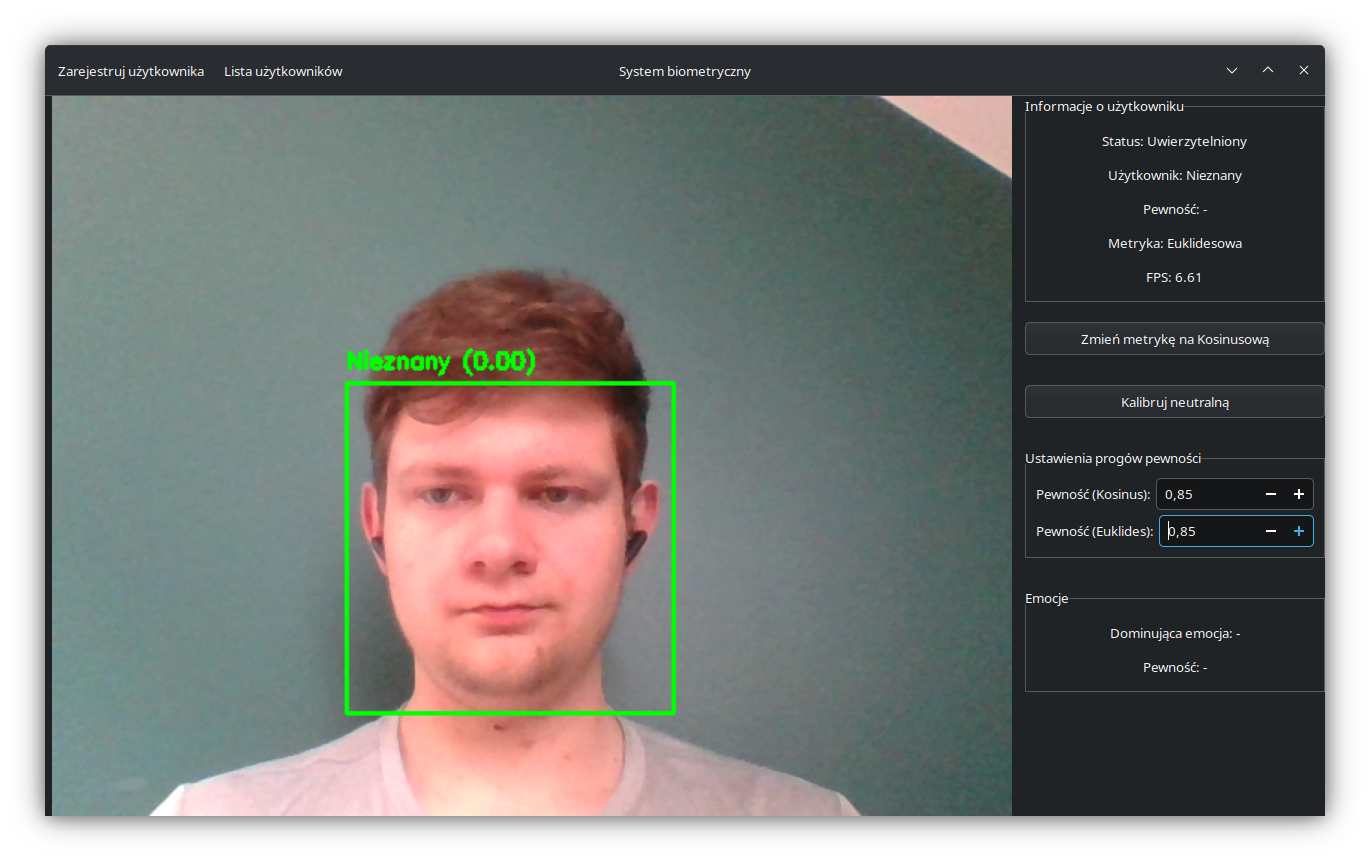
\includegraphics[width=\textwidth]{figures/uzytkownik_niezidentyfikowany_ponizej_progu.png}
    \caption{Interfejs w momencie wykrycia twarzy, która nie została dopasowana do żadnego zarejestrowanego użytkownika.}
    \label{fig:nierozpoznany}
\end{figure}

\subsection{Optymalizacja wydajności poprzez śledzenie obiektów}
Pełne rozpoznawanie twarzy w każdej klatce wideo jest operacją kosztowną obliczeniowo. Aby zapewnić płynne działanie aplikacji, zaimplementowano mechanizm optymalizacyjny. Polega on na inteligentnym przełączaniu się między dwoma trybami:
\begin{enumerate}
    \item \textbf{Pełne rozpoznawanie}: Wykonywane co \texttt{recognition\_interval} klatek (domyślnie 30) lub gdy w scenie pojawi się nowa osoba. Polega na detekcji wszystkich twarzy, ekstrakcji ich cech i porównaniu z bazą danych.
    \item \textbf{Śledzenie (tracking)}: Po pomyślnym rozpoznaniu użytkownika, system inicjuje szybki algorytm śledzący (w projekcie użyto \texttt{cv2.TrackerKCF\_create}), który w kolejnych klatkach jedynie aktualizuje pozycję ramki otaczającej twarz. Jest to operacja znacznie mniej wymagająca obliczeniowo.
\end{enumerate}
Logika przełączająca między tymi trybami znajduje się w metodzie \texttt{authenticate\_user} (listing \ref{lst:auth_user_opt}) i znacząco redukuje obciążenie procesora.

\lstinputlisting[language=python, caption={Fragment logiki optymalizacyjnej w metodzie \texttt{authenticate\_user}}, label={lst:auth_user_opt}, linerange={317-338}]{src/biometric_system.py}

\section{Autorski algorytm analizy emocji}
Moduł \texttt{emotion\_analyzer.py} stanowi w całości autorskie rozwiązanie problemu analizy emocji. Mimo iż do detekcji siatki punktów na twarzy wykorzystano bibliotekę MediaPipe, cała interpretacja tych danych jest zaimplementowana od podstaw.

\subsection{Kalibracja spersonalizowanego modelu}
Kluczową implementacją jest mechanizm kalibracji, który pozwala dostosować system do unikalnej anatomii twarzy każdego użytkownika. System nie opiera się na uniwersalnym modelu emocji, lecz tworzy spersonalizowaną \textbf{linię bazową (baseline)}.

Proces kalibracji, uruchamiany przez użytkownika przyciskiem \textit{Calibrate neutral face}, polega na zebraniu określonej liczby próbek (domyślnie 25) jego neutralnego wyrazu twarzy. Dla każdej próbki obliczany jest zestaw cech geometrycznych (opisanych w kolejnej sekcji). Po zebraniu wszystkich próbek system oblicza ich średnią, która staje się punktem odniesienia (linią bazową) dla tego użytkownika. Proces ten jest implementowany w metodzie \texttt{start\_calibration} w klasie \texttt{EmotionAnalyzer}.

Linia bazowa jest następnie zapisywana w sesji użytkownika, dzięki czemu kalibrację wystarczy przeprowadzić tylko raz. Takie podejście sprawia, że system jest znacznie bardziej odporny na indywidualne różnice w budowie twarzy i precyzyjniej wykrywa subtelne zmiany w mimice.

\subsection{Geometryczna analiza cech}
Emocje są rozpoznawane na podstawie zmian w geometrii twarzy. Zaimplementowano funkcję \texttt{\_calculate\_distances}, która oblicza znormalizowane odległości i stosunki między punktami charakterystycznymi, odpowiadające konkretnym ruchom mięśni twarzy, np.:
\begin{itemize}
    \item \textbf{Uśmiech}: Stosunek odległości między kącikami ust a szerokością ust.
    \item \textbf{Zdziwienie}: Stopień otwarcia oczu i ust.
    \item \textbf{Złość}: Odległość między brwiami (zmarszczenie).
\end{itemize}

\subsection{Wnioskowanie oparte na regułach i progach}
Ostateczna klasyfikacja emocji odbywa się za pomocą autorskiego systemu regułowego. Najpierw obliczane są \textbf{odchyłki} bieżących cech geometrycznych od zapisanej linii bazowej. Te odchyłki są normalizowane, aby uniezależnić je od wielkości twarzy w kadrze.

Następnie znormalizowane wartości są mapowane na poszczególne kategorie emocji za pomocą predefiniowanych wag, przechowywanych w słowniku \texttt{EMOTION\_WEIGHTS} (listing \ref{lst:emotion_weights}). Każda cecha (np. \texttt{'smile'}) wpływa na wynik jednej lub więcej emocji (np. \texttt{'HAPPY'}).

\lstinputlisting[language=python, caption={Fragment wag emocji w pliku \texttt{emotion\_analyzer.py}}, label={lst:emotion_weights}, linerange={56-64}]{src/emotion_analyzer.py}

Wynikiem jest rozkład prawdopodobieństwa dla każdej z emocji. Emocja z najwyższym wynikiem jest prezentowana w interfejsie użytkownika, co widać na rys. \ref{fig:gui}. Takie podejście, choć prostsze od głębokich sieci neuronowych, jest w pełni interpretowalne i niezwykle wydajne, co jest kluczowe w zastosowaniach czasu rzeczywistego.

\subsection{Implementacja analizy geometrycznej}
Implementacja funkcji \texttt{\_calculate\_distances} (listing \ref{lst:calc_dist}) z modułu \texttt{emotion\_analyzer.py} oblicza kluczowe cechy geometryczne na podstawie siatki twarzy, co stanowi fundament dla systemu regułowego wnioskującego o emocjach.

\lstinputlisting[language=python, caption={Implementacja funkcji \texttt{\_calculate\_distances}}, label={lst:calc_dist}, linerange={102-141}]{src/emotion_analyzer.py}

\subsection{Wątek przechwytywania wideo}
Klasa \texttt{CaptureThread} (listing~\ref{lst:capture_thread}) działa w oddzielnym wątku, odpowiadając za pobieranie klatek z kamery i delegowanie zadań rozpoznawania. Takie podejście zapobiega blokowaniu interfejsu graficznego, zapewniając płynność działania aplikacji.

\lstinputlisting[language=python, caption={Klasa \texttt{CaptureThread} z pliku \texttt{main.py}}, label={lst:capture_thread}, linerange={23-53}]{src/main.py}

\subsection{Rejestracja nowych użytkowników}
Metoda \texttt{register\_face} (listing~\ref{lst:register_face}) odpowiada za przetworzenie obrazu, wyekstrahowanie wektora cech twarzy i zapisanie go w bazie danych w celu umożliwienia przyszłego uwierzytelniania.

\lstinputlisting[language=python, caption={Metoda \texttt{register\_face} z pliku \texttt{face\_utils.py}}, label={lst:register_face}, linerange={81-177}]{src/face_utils.py}





